% Nallino, Part I p. 234: the epicycle of the Moon at the lunar eclipses of 883 and 901, redrawn from the print:
% the epicycle about A; the straight line from its top Q through A to the Earth E, the radius AL and the line LE,
% the angle QAL being the true anomaly; the two lines meet at E where their measured ink ends; the bold italic
% letters. Measured on the scan (_intake/latin/tools/fig234).
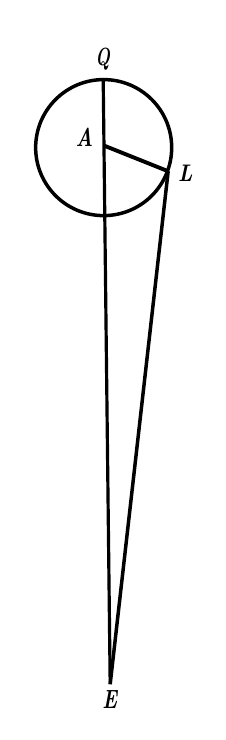
\begin{tikzpicture}[x=0.9914pt,y=-0.9914pt,line cap=butt,every node/.style={font=\fontsize{11}{11}\bfseries\itshape\selectfont,inner sep=0pt}]
\useasboundingbox (0,0) rectangle (62.00,249.20);
\draw[line width=1.26pt] (27.70,43.71) circle[radius=24.79];  % the epicycle about A
\draw[line width=1.15pt] (27.53,18.92) -- (30.07,239.30);  % QE, through A
\draw[line width=1.41pt] (27.79,42.97) -- (51.21,52.33);  % AL
\draw[line width=1.26pt] (51.21,52.33) -- (30.07,239.30);  % LE
\node at (27.35,11.50) {\normalfont\fontsize{11}{11}\bfseries\itshape\selectfont \resizebox{5.30pt}{6.16pt}{Q}};
\node at (20.66,40.22) {\normalfont\fontsize{11}{11}\bfseries\itshape\selectfont \resizebox{6.33pt}{6.40pt}{A}};
\node at (57.44,53.20) {\normalfont\fontsize{11}{11}\bfseries\itshape\selectfont \resizebox{5.20pt}{5.94pt}{L}};
\node at (29.88,244.78) {\normalfont\fontsize{11}{11}\bfseries\itshape\selectfont \resizebox{5.33pt}{6.54pt}{E}};
\end{tikzpicture}
